\graphicspath{{../images/ch5/}}	% Image directory


\chapter{Resistive pulse studies of cancer cell deformability}
\label{chap:cell}

	

	\section{Background \& Theory}
	      
		One of the most important applications in microfluidic technology today is the study of cell populations. The most important tool for studying cell properties is the flow cytometer, invented in 1965 by Fulwyler \cite{Fulwyler1965}, and is conceptually the follow up to Coulter counters which can be considered to be impedance cytometers. Flow cytometers are a mixture of many individual microfluidic elements combined in series, each with its own function. On the sensing side, flow cytometry makes use of measured scattering of laser light as well as detection of fluorescence signals. Dyes are specifically attached to certain types of antibodies, which then may interact with the cell membranes in the suspension. When the cells are pulsed by lasers in the laser light, it stimulates emission of specific dyes, which can be measured to determine which antibodies have interacted with the cell. This type of information is incredibly value in determining phenotypic and classification information for the cells. Furthermore, the information garnered from real-time cytometry information can be used to sort cells in real time, in a system known as fluorescence activated cell sorting system (FACS). Cell cytometry is the workhorse of modern day molecular and cellular biology studies, but suffers from the fact that it is a label-dependent method due to the introduction of the dyes. Such labels can adversely affect the the cells' viability that prevents them from being used in a post-interrogation analysis, even after being separated by a system like FACS. Additionally, flow cytometry requires the use of costly fluorescent reagents and skilled technicians that must be present to perform the measurement and to ensure proper calibration of the fluorescence signal \textit{via} the use of fluorescent beads \cite{Gosset2012} (DiCarlo PNAS).
	
		While flow cytometry focuses on the measurement of cells' interactions with specific antibodies, another dimension often not thought of is the cells' mechanical properties, such as their size, shape, deformability, and deformability dynamics \cite{Lin2017} (DiCarlo paper in Nature 2017). Since their discovery, we've known that a wide variety of cell sizes exist, but more recently scientists have focused on the difference in the mechanical stiffness of cells. Cell stiffness has been shown to vary from cell to cell, and even between various stages in cells' mitotic cycles. As a concrete example, cancer cells are known to be generally `squishier' than non-cancerous cells. For these reasons, developing a method of probing the mechanical stiffness of cells is highly desirable for cell characterization applications, and serve as a complementary cell phenotyping platform to deformability cytometry.
		
		In order to measure the stiffness of an object, it must be subjected to constrained forces and its response measured. Probably the most straight forward way of doing this is by directly applying a mechanical force on the cell, for example by using an atomic force microscopy (AFM) probe to directly press on the cells and measure the resultant recoil force felt by the AFM's cantilever, which is directly related to the Young's modulus of the cell. Other similar methods exist, and while they are very accurate and easily interpretable, they suffer from an excruciatingly slow throughput. For instance, using AFM for cell deformation measurement can take a few minutes per cell. For cell applications a high throughput is necessary, and therefore these applications are not feasible for discovering cell population statistics.
		
		Another method of measuring cell deformability is with microfluidics platforms. Cells passing quickly through narrow constrictions are subjected to large, anisotropic hydrodynamic forces, and these forces can induce a measurable particle deformation. The advantage of this type of method is its extremely large throughput; rather than spending several minutes per particle as in measurements conducted with AFM, thousands of cells per second can be measured in microfluidic platforms. Even within the narrow field of microfluidic-based deformability cytometry, there are multiple types of platforms. Probably the most conceptually simple is a standard microfluidic channel that tightly confines cells passing through it. Due to anisotropies in the hydrodynamic stresses and strains around the particle, it will deform even in a uniformly shaped channel.
		
		In traditional microfluidic methods of measuring cell deformability, direct imaging is used to determine the cell shape across different frames in the video, which corresponds to the hydrodynamic load it is under. However, for the high throughputs that are the reason why people use microfluidics, camera imaging must be performed very quickly. This requires the use of a high-speed camera used in conjunction with an optical microscope, usually shooting at a minimum of $\SI{10000}{fps}$. When combined with an optical microscope, such high-speed cameras are capable of capturing cell deformations with high spatial and temporal resolution, and are even capable of resolving the cells' deformation dynamics \cite{DiCarlo2017}. Currently high-speed camera imaging is by far the most popular method of capturing cell deformations, but it comes with two serious disadvantages. First, the camera itself adds a large cost to the apparatus, and will likely dwarf the price of any other component in the deformability cytometer. Second, imaging data is inherently highly multidimensional and computationally expensive to analyze. As a result, online analyses conducted during the run of the experiment are usually not possible at the flow rates that these experiments operate at. While the data can still be stored, processed, and analyzed later, offline analysis does not allow for real-time separation, one of the most highly desirable applications of this type of metrology.
		
		Instead of using camera imaging, one can instead imagine trying to employ resistive pulse (RP) to measure the deformability of particles. In terms of practicality, RP is far more computationally light than imaging data, as the following order of magnitude estimate shows. First, consider the data bandwidth in high-speed imaging. Passage through a deformability cytometry system may consist of $\sim100$ frames, each with a resolution of perhaps $100x50$ 8-bit grayscale valued pixels. As a result, a single translocation is described by $\SI{500}{kB}$ worth of data. At a rate of $1000$ particles per second, this corresponds to a raw data throughput of $\SI{500}{MB/s}$ of data that must be processed. Finally, in a common image processing algorithm the number of computations performed on each pixel is probably greater than one; identifying the shape of an object in a frame certaintly consists of multiple serial image processing steps. Although this is just an estimate, it conveys the point that high-speed imaging is not amenable to online analysis, especially at the throughputs that are desired for these types of calculations. On the other hand, consider a resistive pulse analysis: under the same criteria described above, an RP data stream being sampled at $\SI{1}{MHz}$ will consist of a data throughput of only $\SI{1}{MB/s}$, a factor of $500$ decrease in raw data throughput. Furthermore, the types of operations needed to extract deformability information from the raw RP signal are also computationally light relative to image processing techniques.
		
		While it is apparent that resistive pulse is computationally cheaper than imaging analysis, it is most important to demonstrate that deformability can actually be measured via RP sensing. In chapter 4 of this dissertation, we discussed the equations for the resistive pulse amplitudes of ellipsoidal objects. For cells that are spheroidal in their unloaded state, ellipsoids are reasonable geometries to expect for the deformation shape in the loaded state, at least as an approximation. If we consider a straight ion conducting channel with an ellipsoidal particle inside it, the aspect ratio and orientation of the particle greatly affects the ionic resistance of the system. Under the assumption that the particles take on ellipsoidal geometries, the shapes will be described as being prolate, oblate, or spherical with respect to the channel's axis. Oblate geometries correspond to a flattening along the channel's axis, and prolate geometries are an extension along the channel's axis. The difference in the measured resistive pulse amplitude of these particles is given by the following equation:
		
		\begin{equation}\label{eq:ellipsoiddI}
			\frac{\Delta I}{I_{p}}=f_{\parallel}\frac{v}{V},
		\end{equation}
		
		where $v$ and $V$ are the volume of the particle and channel, respectively, and $f_{\parallel}$ is a constant known as the `shape-factor', which depends on the aspect ratio of the ellipsoid. 
		
		\begin{figure}
			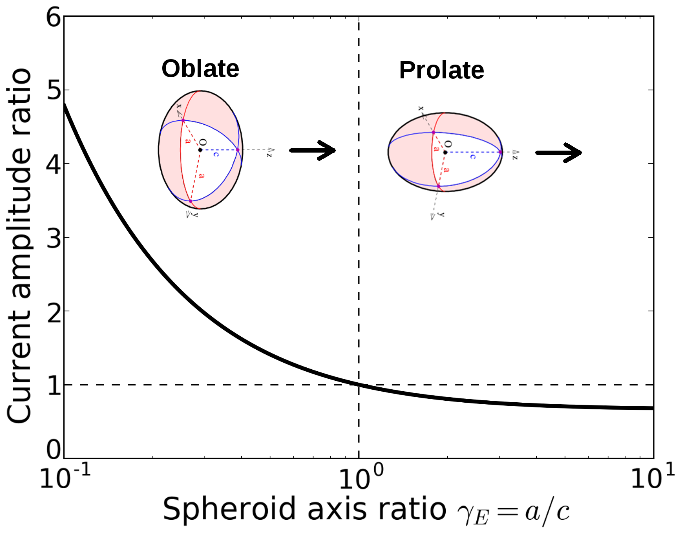
\includegraphics[width=0.5\textwidth]{dIellipsoid.png}
			\caption{\textbf{Resistive pulse amplitude $\Delta I/I_{p}$ for equal volume spheroidal objects relative to a sphere.} The polar axis of the particle is aligned with the channel's axis, so that oblate geometries correspond to motion along the channel axis. The values come from equation \ref{eq:ellipsoiddI} when the correct shape factor $f_{\parallel}$ is applied.}
		\end{figure}

		
		For spheres, $f_{\parallel}=1$, and for prolate and oblate spheroids, $f_{\parallel}<1$ and $f_{parallel}>1$, respectively. Figure \ref{fig:dIellipsoid} shows plots of the RP amplitude $\Delta I/I_{p}$ for ellipsoids of the same volume but different aspect ratios, relative to a sphere. The plot reveals that even for modest deformation, for instance a stretching ratio of $2/3$, a mildly oblate ellipsoid, the increase in $\Delta I/I$ is nearly $30\%$. Similarly, the current $\Delta I/I$ changes for prolate geometries, although to a lesser degree.
		
		As mentioned previously, there are many possible types of high throughput microfluidic systems than can induce cell deformations. We devised a method that has been shown to be capable of inducing bidirectional deformations (prolate and oblate). The key to understanding the channel geometry is to understand the primary hydrodynamic forces that work on a cell and deform it in extensional, i.e. accelerating and decelerating flows. When a cell transitions from a region of high local fluid velocity to low local fluid velocity, there is a greater magnitude of normal stress forces on the back of the particle than on the front. Consequently, the particle is pushed into a laterally elongated state, corresponding in our model to the oblate geometry. Oppositely, when the particle makes the transition from a slow to fast region, the net forces pulling the particle forward are greater than the forces pushing it from behind, elongating it in its direction of motion. This corresponds to the prolate shape configuration. According to this model, one can induce bidirectional shape changes in passing particles by having transitions between regions of slow and fast local fluid flow, and vice versa. This criterion allows for multiple possibilities, but the geometry chosen for our system is described by a channel having a central cavity, but otherwise with a straight cross-section. As the cell enters the microchannel, it accelerates and is pulled in, and in the process deforms into a prolate shape. When the cell arrives at the central cavity, the fluid flow is slower and the particle decelerates, becoming oblate. At the end of the cavity, the particle again undergoes an acceleration and deforms back into its prolate shape. Figure \ref{fig:channelscheme} shows an example image of one of the channel geometries used in this study, along with a scheme showing the deformation modes that occur in each region of the channel.
		
		Although the deformation dynamics are undoubtedly complicated, to first order we seek to find the aspect ratio of the approximate ellipses $a/b$ at various points in the channel. The aspect ratio will remain the same at all points for completely non-deforming particles, but will vary according to the above model for deforming particles, and to a greater degree for the most deformable particles. For the scheme shown in Fig. \ref{fig:channelscheme}, the expected aspect ratio $a/b$ as a function of the axial position adheres to the motif shown in Fig. \ref{fig:aspectmotif}. Besides size, the observables of interest might be the minimum and maximum aspect ratios, or perhaps the ratio of the minimum and maximum aspect ratios which would reflect the general elasticity properties of the cells. However, in the RP signal the actual deformation of the particles would be reflected in the changes in the measured $\Delta I/I_{p}$ signal \textit{relative to the expected $\Delta I/I_{p}$ of a completely non-deforming spherical particle of the same volume}. This means in the narrow regions where a prolate elongation occurs the current amplitude $\Delta I/I_{p}$ would be \textit{decreased}, while in the central cavity where the particle assumes an oblate geometry the signal would be \textit{increased}. Figure \ref{fig:RPmotif} shows an example RP event for a particle passing through the cavitated channels, and the distortion of the RP signal corresponding to the model described above. Therefore, the observable of interest might be the ratio of the maximum in the signal (minimum $\Delta I/I_{p}$) and either of the two minima in the signal (maximum $\Delta I/I_{p}$), which would be a proxy measurement for the ratios of the aspect ratios calculated directly from imaging data. For larger deformations, this ratio would increase as the signal distortion motif in Fig. \ref{fig:RPmotif} shows.
		
	\section{Experiment and data analysis}

		In order to test the concept of cell deformability cytometry with the channel geometry described above and using RP, we ran microfluidic experiments with cancer cells. Although the ultimate goal of this sensor will be to perform deformability cytometry with the RP signal alone, in order to test the method it is necessary to have a high-speed camera. In the following sections we describe the complete experimental set up, the software used to control the experimental instrumentation, and the data processing and analysis steps that take place after the experiment. To date, the experiments performed have primarily been focused on analyzing the optical data in the experiments, since measuring their deformability optically is a prerequisite for determining it via the RP signal.
	
		\subsection{Experiment and instrumentation control}
		
			The entities involved in the experiments include the microfluidic channels, the cells and the suspension media that holds them, a syringe pump to drive the suspension through the systems, a microscope and high-speed camera used to take the images, the data acquisition card (DAQ) that acquires the RP signal, a central control computer used to run the experiments,  and various other miscellaneous pieces of equipment. A more in-depth description of these components and the roles they play in the experiment is as follows.
			
			\begin{figure}
				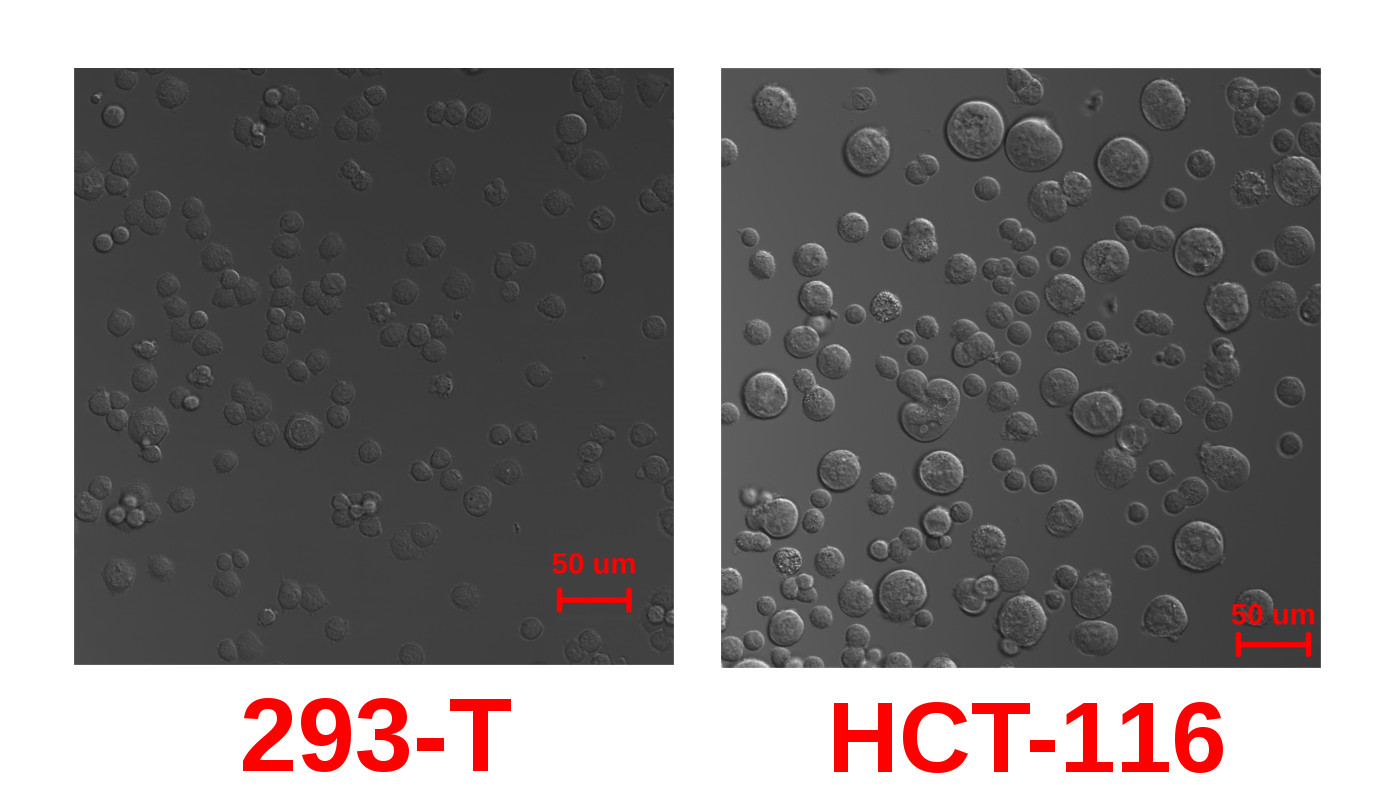
\includegraphics[width=\textwidth]{celllines.jpg}
				\caption{\textbf{Confocal images of 293-T (left) and HCT-116 (right) cells.} Scale bars are $\SI{50}{\mu m}$ long.}
				\label{fig:celllines}
			\end{figure}

			
			First, we start with the cells. Three human cell lines were provided for the experiments, chosen for the variety of deformation and size properties they exhibit. The cell lines are HCT-116 (colorectal cancer), 293-T (derived from human embryonic kidney cells), and THP-1 (monocytes). Images of the HCT-116 and 293-T cells are shown in Fig. \ref{fig:celllines}. The cells are filtered and diluted to a concentration of $0.5\times10^{6}/$mL or $1\times10^{6}/$mL in a solution of HBSS, a relatively highly conductive biocompatible buffer. In most experiments, the solution was doped with methylcellulose, another biocompatible component that increases the viscosity of the solution, which should promote cell deformations. Pluronic, a biocompatible surfactant, is added at $0.1\%$ concentration by volume.
			
			\begin{table}
				\begin{center}
				    \begin{tabular}{lrc}\hline
						Step name & Instrument & Parameters \\
						\hline
						Preprocess cleaning & Isoproponal & \\
						Wafer dehydrate & Dry oven & $95^{\circ}$C, $\SI{30}{min}$ \\
						First spin & Laurell spinner & (parameters) \\
						Second spin & Laurell spinner & F \\ \hline
						Soft bake (cold) & Hot plate & $65^{\circ}$C, $\SI{1}{min}$ \\
						Soft bake (hot) & Hot plate & $95^{\circ}$C, $\SI{5}{min}$ \\
						UV flood exposure & AMV & $\SI{52}{seconds}$ (intensity varies, adjust accordingly) \\
						Post-exposure bake (cold) & Hot plate & $65^{\circ}$C, $\SI{1}{min}$ \\
						Post-exposure bake (hot) & Hot plate & $95^{\circ}$C, $\SI{5}{min}$ \\
						SU8 develop & SU8 develop solution & $\SI{5}{min}$ soak, with periodic agitation of solution \\
						SU8 developer rinse & SU8 developer solution & \\Soft bake (hot) & Hot plate & $95^{\circ}$C, $\SI{5}{min}$ \\
						Post-photolithography bake & Hot plate & $95^{\circ}$C, $\SI{2}{hours}$ \\
						\hline
						PDMS preparation & Sylgard-184 and curing agent & 10:1 by volume Sylgard-184 to curing mix \\
						PDMS degassing & Vacuum & $\SI{30}{min}$ \\
						PDMS cure on SU8 mold & Hot plate & $75^{\circ}$C, $\SI{150}{min}$ \\
						PDMS-glass bond & Harrick-Plasma oxygen plasma chamber & $\SI{300}{mT}$, med. power, $\SI{35}{sec}$    
				    \end{tabular}
				    \caption{Class Mark List}\label{tab:devicefab}
				\end{center}
			\end{table}
			
			
			
			
			
			The microfluidic channels are fabricated \textit{via} standard, well-established soft photolithography techniques. Fabrication primarily takes place in a class 10000 clean room of the BiON facility at the University of California, Irvine. First, SU8-2025 photoresist is spun onto a $\SI{4}{inch}$ silicon wafer with the correct rotational speed to achieve a thickness of $\SI{20}{\mu m}$. A transparency with the channel design printed on with a high DPI printer is taped onto the SU8 side of the wafer, which is then exposed to a UV flood lamp. UV light passes through the non-printed parts of the transparency and reaches the SU8 photoresist. Polymer molecules in the exposed areas are cross-linked, resulting in these regions being more stable. The photomask is then removed, and the wafer soaked in SU8 developer solution until the non-crosslinked parts of the channel are completely washed away. The resulting structures left after the SU8 is washed away comprise the device mold. PDMS, a relatively chemically inert elastomer is degassed and then poured over the mold and baked until completely hardened. After curing, the PDMS layer is carefully pulled off the wafer, and individual microfluidic devices are cut out. The inlet and outlet access ports are punched through with a biopsy punch. Finally, the PDMS device and glass slide are treated in an oxygen plasma which temporarily alters the chemical composition of the surfaces, allowing for bonding. After being taken out of the plasma, the glass slide and PDMS layer are quickly but delicately pressed together, resulting in a quick bonding. Table \ref{tab:devicefab} contains a list of the key steps involved in the device fabrication, the particular instrument(s) used in each step, and all main parameters relevant to those instruments operations in this application.
			
			Once the device is fabricated, it is taped onto the glass stage of the optical microscope. The high-speed camera is mounted on to the microscope, where the light is directed instead of into the eyepiece. Plastic tubing, which serves as the fluid access, is inserted into the inlet and outlet ports. Ag-AgCl electrodes are inserted into the tubing as well, as close as possible to the actual microfluidic device. The electronic set up used to make RP measurements consists of a patch clamp amplifier, which in its current configuration merely applies a voltage, and a lower amplification amplifier. This circuit is connected to a BNC breakout box, which connects to the data acquisition card via a parallel data bus, which actually streams the measured RP data. A syringe containing the particle solution is inserted into the inlet tubing with a luer lock configuration, and the syringe is mounted onto a syringe pump which is used to drive the solution through the channel. Finally, the syringe, high-speed camera, and data acquisition card are all connected into a central control computer which is used to command the three instruments and save their data locally. Figure \ref{fig:hardwarescheme} shows a scheme of the hardware implementation used for the experiment.
			
			In order to control the three insruments and save data, a graphical user interface (GUI) program was written. The program was written in C++ and the Qt Framework, and uses threading to ensure asynchronous operation of the three instruments, as well as the controls in the GUI itself. Communication protocols used were specific to each of the hardware instruments. The software communicates with the syringe pump \textit{via} a serial RS-232 communications protocol. Communication with the high-speed camera occurs over TCP/IP protocol over a 1 Gb ethernet line, with instructions specific to the camera's manufacturer. Lastly, the DAQ card is controlled via the niDAQMX software library. The software allows the user to perform all operations on the syringe pump remotely. When not recording, the software displays live images from the camera feed that show the view through the microscope. The user may also change the camera's recording parameters such as frames per second, exposure rate, and pixel resolution, and when ready, to record videos and save the data to the computer after recording. Similarly, the software also displays the RP data stream and can save it as well. Figure \ref{fig:cellcontroller} shows an image of the GUI program; the software is open-sourced and available at https://github.com/tphinkle/cell\_controller.
			
			After the cell suspension is prepared and the experiment set up, data recording occurs. The syringe pump is started so that the solution is driven through the microfluidic channels. The initial `push' of the syringe pump is usually much greater than needed, which serves two purposes. First, it quickly pushes the solution from the syringe pump to the actual device. Sedimentation due to gravity is significant for the cells used here, so a quick start to the experiments is highly desirable in order to ensure high event frequency during recording. The second purpose of pushing solution very rapidly is that it puts the fluid into a turbulent regime. In this regime, the regions of solution adjacent to the exit of the channel display stable turbulent vortical flows, and are very likely to capture cells. These trapped cells provide a target by which to focus the microscope; due to the extremely small size of the channels, even under small latent pressures in the system (i.e., without pushing on the syringe pump), cells move far too quickly to properly focus on, usually staying in the field of view of the camera for only a single frame in the GUI's view. However, while the cells trapped in the vortical flows at the channel's exit are rapidly moving, they do not leave the field of view of the camera and therefore act as a moving target on which to focus the microscope. This unconventional trick has proven absolutely invaluable in the experimental workflow, as the focus required to obtain good camera images of the cells is very sensitive. In unfocused images, while cells may be detected their boundaries are often non-resolvable. After the proper focus has been established, the flow rate is reduced to the desired flow rate that the user wishes to record, and a fixed amount of time is waited to allow the fluid to equilibrate. After this delay, both the RP and camera signal are recorded. While the recording itself is very fast, the data must be transferred to the control computer in order for it to be stored; the onboard camera memory is only sufficient to hold the data of a single recording. The transfer and saving process takes nearly 15 minutes, and over this duration of time the vast majority of cells sediment to the bottom of the tubing and syringe. For this reason, in between data transfers we remove the tubing and syringe and clean them. After recording, the solution is gently mixed to resuspend the cells, and the process of pushing the solution, refocusing the microscope, and recording is repeated. Experiments are repeated in this way for different cell lines, channel geometries, and fluid flow rates. Following the experiments, data is immediatley backed up redundantly to external storage drives where it remains until it is ready for post processing and analysis.
		
		
		
		\subsection{Data analysis}
			
			The data generated from these experiments includes the imaging data from the camera and the resistive pulse data. In order to analyze this unique combination of data sets, a library called pore\_stats was written in Python. pore\_stats was primarily written for the purpose of analyzing resistive pulse data, however image processing functions were added to analyze the data from these hybrid RP-IM experiments. Pore\_stats is discussed in greater detail in chapter \ref{chap:rpim}
			
			The primary observable of interest in this experiment is the shape of the particle. There is no single way of defining the shape of an object, but because we are interested in comparing the RP signals of cells with the theoretical RP amplitudes of ellipses, we determine the shape of the cell by fitting ellipses to its borders across multiple frames. Thus, the objective in demonstrating deformation optically is to fit ellipses with semi-major axis $a$ and semi-minor axis $b$ to cells across multiple frames and track their change in aspect ratio as they pass through the channel. According to the above model, the cells should oscillate between prolate, oblate, and spherical shapes at various points in the channel, and therefore we expect to observe an oscillation of the determined aspect ratio $\gamma=a/b$ between values $>1$ and values $<1$. The exact shape of the cell is never exactly ellipsoidal, however we find that for most shape configurations it is an adequate approximation.
			
			
			\begin{figure}
				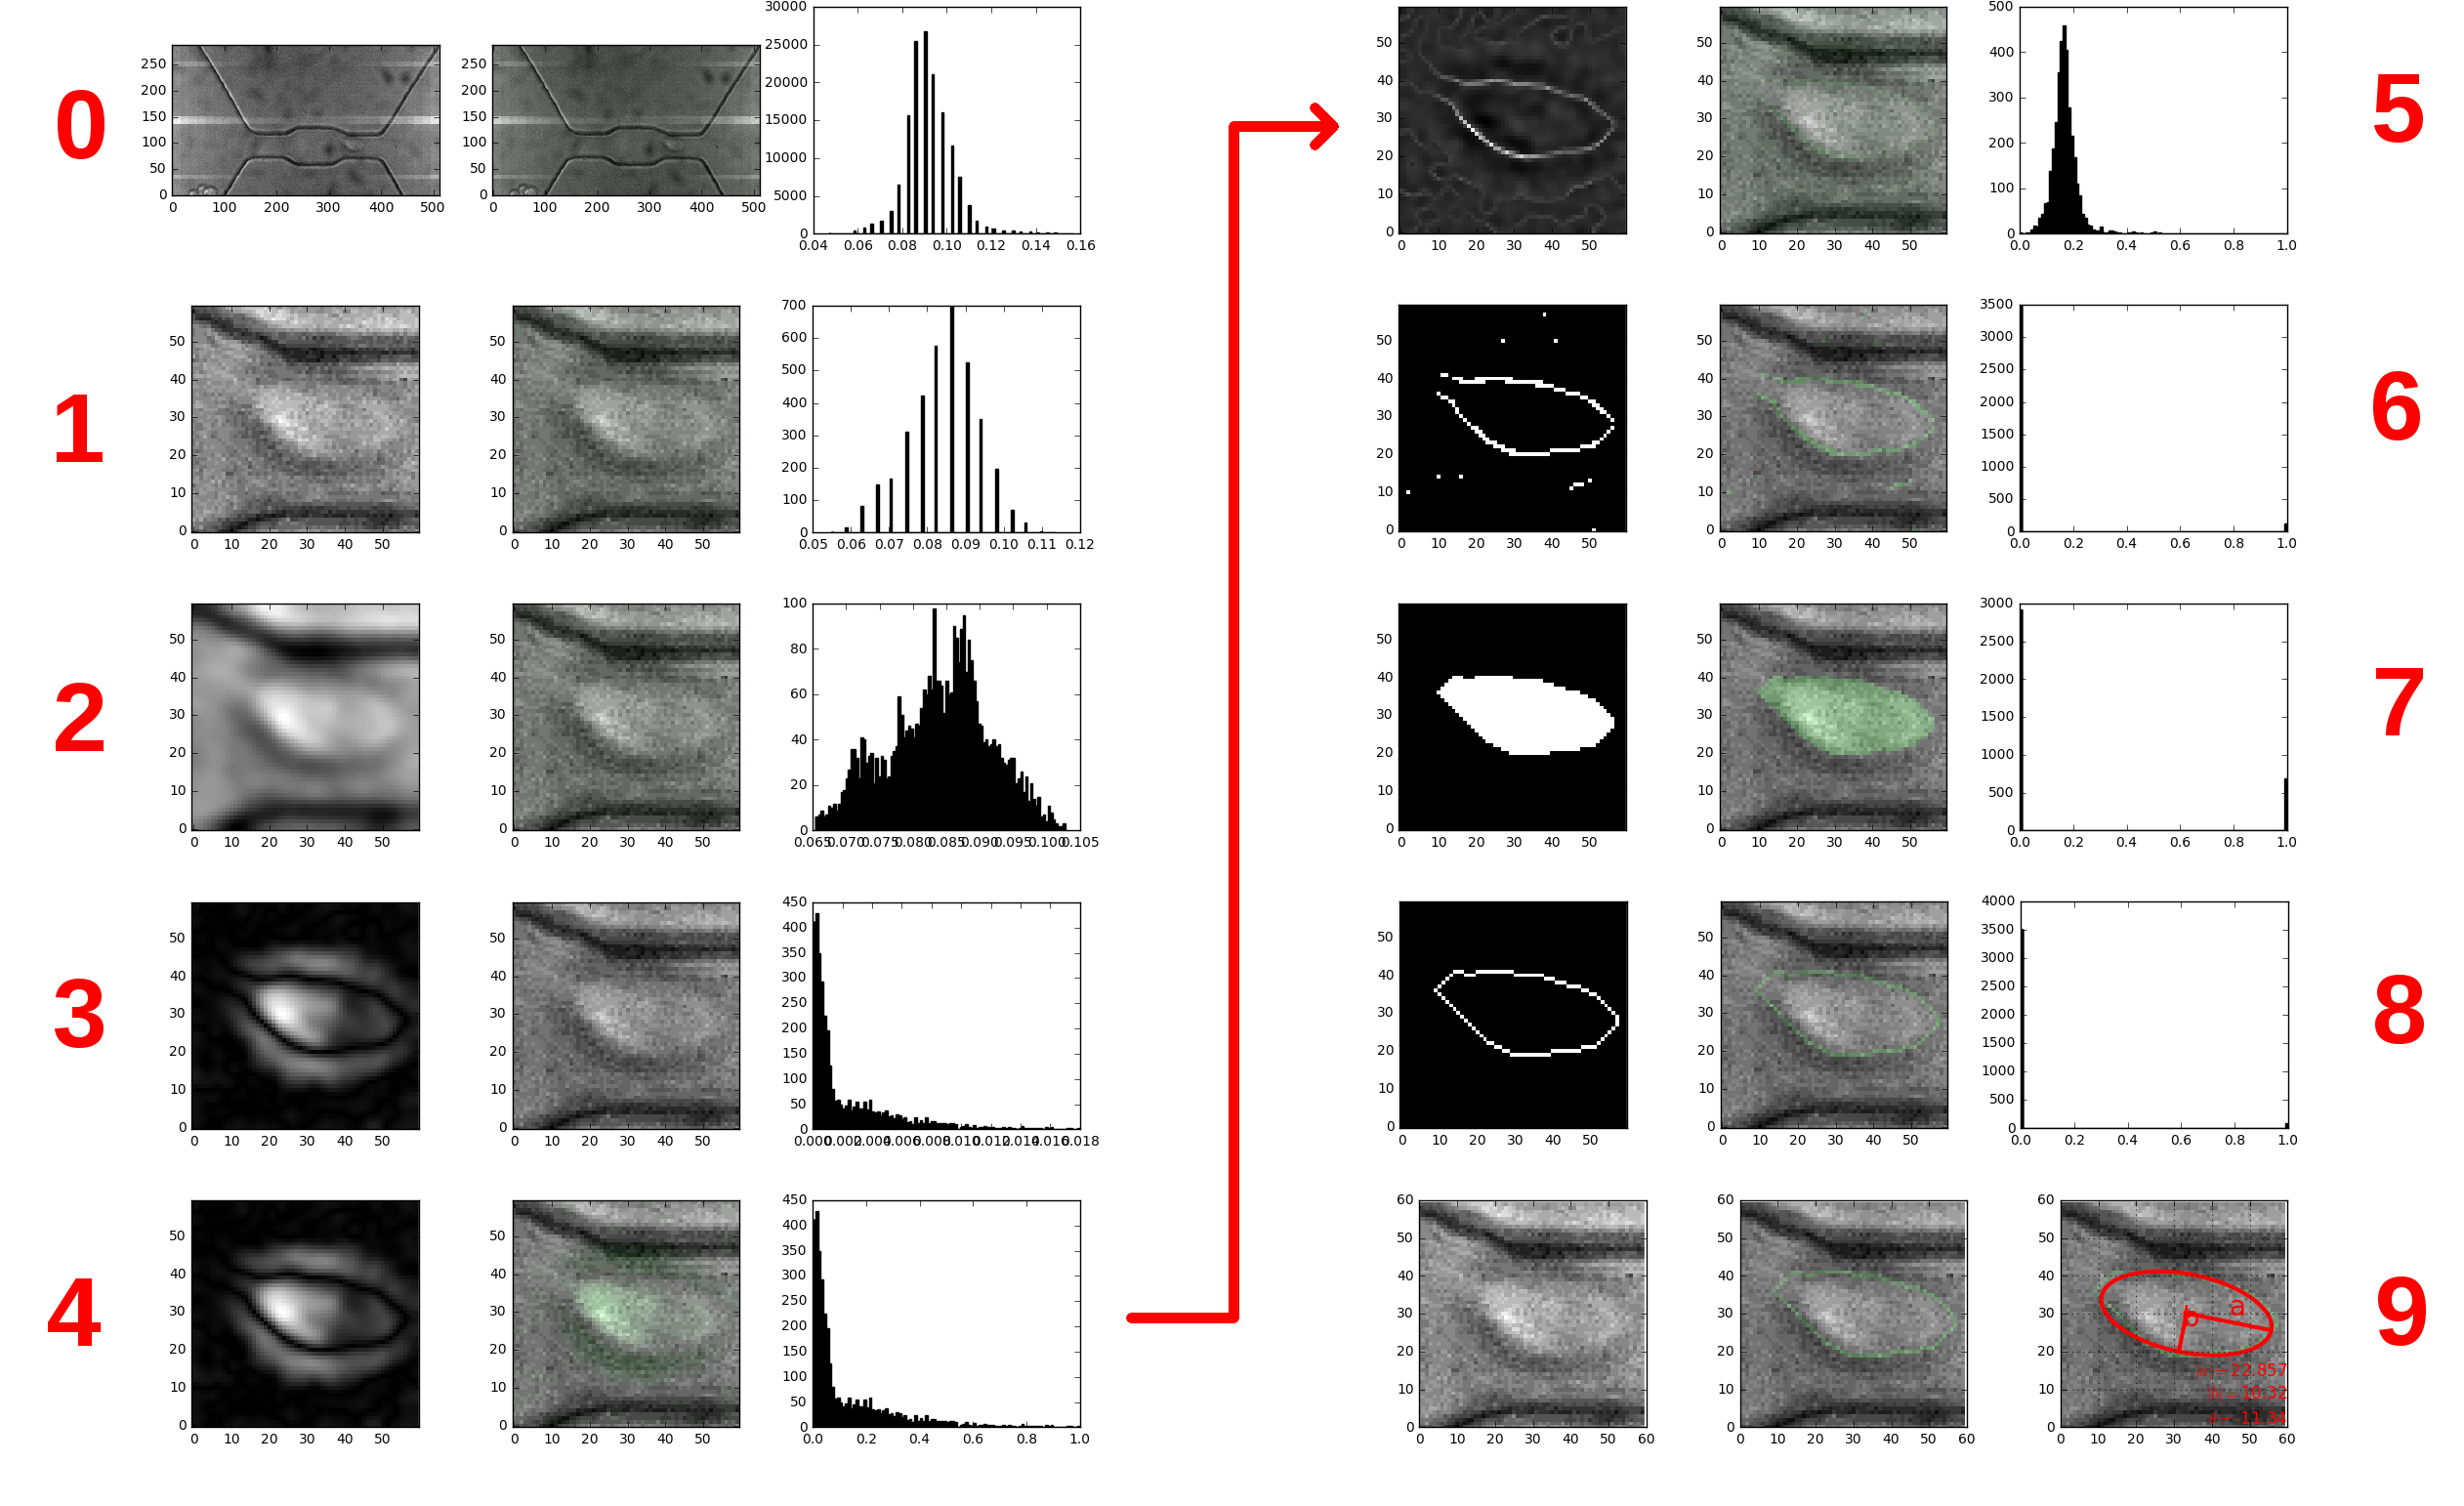
\includegraphics[width=\textwidth]{ellipsefittingprotocol.png}
				\caption{\textbf{Example ellipse fitting protocol for a single detection within a single event.} The left column of each row shows the current image transformation. The central column shows the raw frame with the pixels shaded green with intensity according to the intensity of the pixels in the transformed image. The right column shows pixel intensity in the processed image. \textbf{1: } Raw image. \textbf{2:} Image is cropped in the vicinity of the particle. \textbf{3:} Template image is subtracted off. \textbf{4:} Pixel intensity is rescaled. \textbf{5:} Laplacian derivative. \textbf{6:} Pixel intensity thresholding. Notice the histogram becomes binary distributed. \textbf{7:} Morphological closing of image. \textbf{8:} Image is dilated and subtracted from undilated image, leaving a thin shell around the border of the cell. \textbf{9:} Ellipse is fit to the cell's border.}
				\label{fig:ellipsefittingprotocol}
			\end{figure}

			
			
			While the ellipses could be fit manually by determining the width and height of the channel in each frame, the number of cells observed prohibits this manual measurement. Instead, we devise an image processing pipeline that starts with the raw camera data and results in a calculation of the ellipse fits for every single detection and every single particle passing through the channel. The pipeline works as follows. First, cells are detected in individual frames via a template subtraction method. Then, cells are tracked across frames using a minimum distance approach. These two methods are described in greater detail in chapter \ref{chap:rpim}. After a list of events is determined, ellipses need to be fit to the image of the cell in each frame. A number of preprocessing steps is required to transform the image to a form where this ellipse fitting is possible. One possible ellipse fitting protocol is shown in Fig. \ref{fig:ellipsefittingprotocol}. All processing protocols must reduce the image down to a binary form where the only pixels highlighted are the pixels on the exact boundary of the cell. Operations common to most processing protocols are template subtraction, Gaussian blurring, Laplace derivative transformation, thresholding, and morphological operations such as binary dilation, erosion, and closing. The end result is shown in Fig. \ref{fig:ellipsefittingprotocol}, row 9. Fitting an ellipse to the particle in each frame is useful because many properties of the particle and its translocation can be determined via the ellipse fits. For instance, ellipse fitting yields accurate determination of the central position of the particle, which can be used to accurately determine its trajectory and velocity. Furthermore, once the ellipse is obtained for every frame it is easy to calculate the aspect ratio of the particle during the course of its trajectory and compare with the expectations of the model proposed earlier (Fig. \ref{fig:deformationmotif}.
			
			
	
	\section{Results \& Discussion}
	
		\begin{figure}
			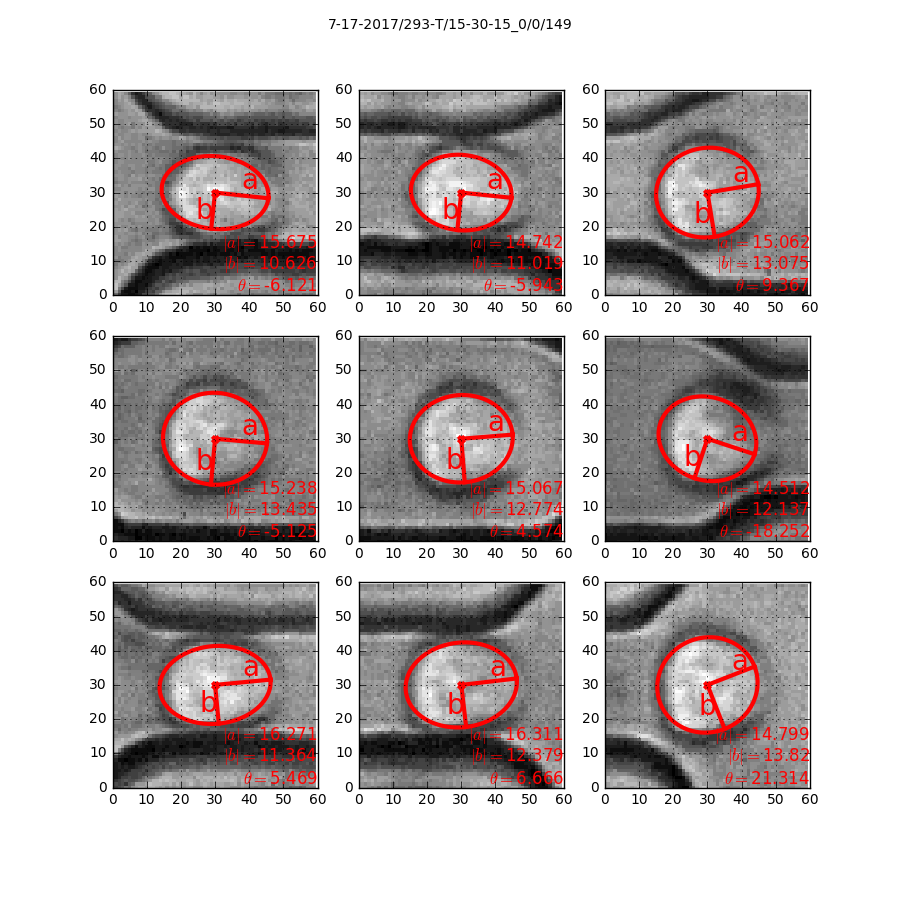
\includegraphics[width=0.5\textwidth]{ellipses.png}
			\caption{\textbf{Ellipse fits for a 293-T cell passing through a $15-30-15 \mu\mathrm{m}$ channel at various positions.} Notice that in the narrow portions of the channel the particle assumes a prolate (axially-elongated) shape, while in the central cavity it assumes an oblate (laterally-elongated) shape, in agreement with the motif presented in Fig. \ref{fig:deformationmotif}}.
			\label{fig:ellipses}
		\end{figure}

	
		The most important question to be answered in the experiments is whether the cells actually deform according to the model proposed. In order to answer this question, we examined specific events to look at their change in aspect ratio as they pass through the channel. Many events consistently show a deformation pattern that subscribes to the model, as shown in Fig. \ref{fig:ellipses}. On the other hand, there were many events that showed modest to little deformation. However, this result is not unreasonable; our model does not suggest that all cells must deform, and indeed there may be cells that are quite resilient to deformations, or cases where the hydrodynamic forces were insufficient to generate significant deformation. However, we never observe a trend opposite to the deformation mode posited, i.e. an oblate-to-prolate transition rather than a prolate-to-oblate transition. This observation suggests that, while the magnitude of the effect may be low in some cases, the effect still occurs.

		

		
		


%%% Local Variables: ***
%%% mode: latex ***
%%% TeX-master: "thesis.tex" ***
%%% End: ***
